
% A first, optional argument in [ ] is the title as displayed in the table of contents
% The second argument is the title as displayed here.  Use \\ as appropriate in
%   this title to get desired line breaks
\chapter[Introduction]{Introduction}

\section{Background}

This dissertation investigates the behavior of the plasmasphere and tests the ability to forecast space weather events based on said behavior. This chapter introduces the major connections the plasmasphere has with the magnetosphere and radiation belts, as well as how their individual processes are interdependent.  It then explores previous attempts to statistically model the magnetosphere and plasmasphere.

\subsection{Magnetosphere}

\subsubsection{Discovery}
The dynamic processes of Earth's magnetosphere and their various impacts on the planet and its inhabitants have been studied for centuries: from Celsius and Hiorter who noted a correlation between compass orientation and aurora \citep{Maunder} to the Carrington event in 1859 that established the connection between solar output and electromagnetic effects on Earth \citep{Carrington}. 

It was not until Van Allen performed his rocket sounding and satellite measurements of high altitude cosmic rays, finding the eponymous Van Allen Radiation Belt, that the structure of the magnetosphere was generally accepted to be more complex than that of a basic dipole magnet \citep{MagnetoHistory}. \cite{Gold1959RingCurrent} showed that charged particles captured from the solar wind plasma are broken into constituent parts that drift in opposing directions around the Earth, leading to a deeper understanding of the behavior the magnetosphere and its interconnectivity with structures both inwards and outwards.

The overall magnetospheric system is portrayed in Figure \ref{RingCurrentFigure}, showing where the solar wind interacts with the bow shock, the magnetopause, and finally the plasmasphere, as well as the overall structure this creates. Each of these components is described in a subsection of this chapter.

\begin{figure}[htp]
	\centering
	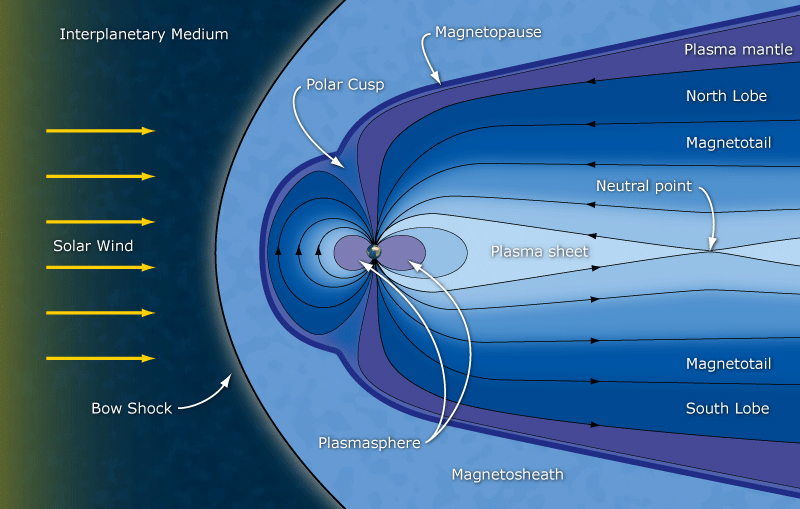
\includegraphics[scale=0.5]{{Figures/MagnetoOverview.jpg}}
	\caption{Overview of the magnetosphere and plasmasphere \citep{MagnetosphereOverallFigure}}
	\label{RingCurrentFigure}
\end{figure}

The inner magnetosphere, where this dissertation is primarily focused, is composed of three main constituent parts: the plasmasphere, the ring current, and the radiation belts, all of which are shown in Figure \ref{fig:magnetosphereoverview}. This helps illustrate how the parts are not always spatially distinct and, depending on conditions, often overlap.


\begin{figure}[htp]
	\centering
	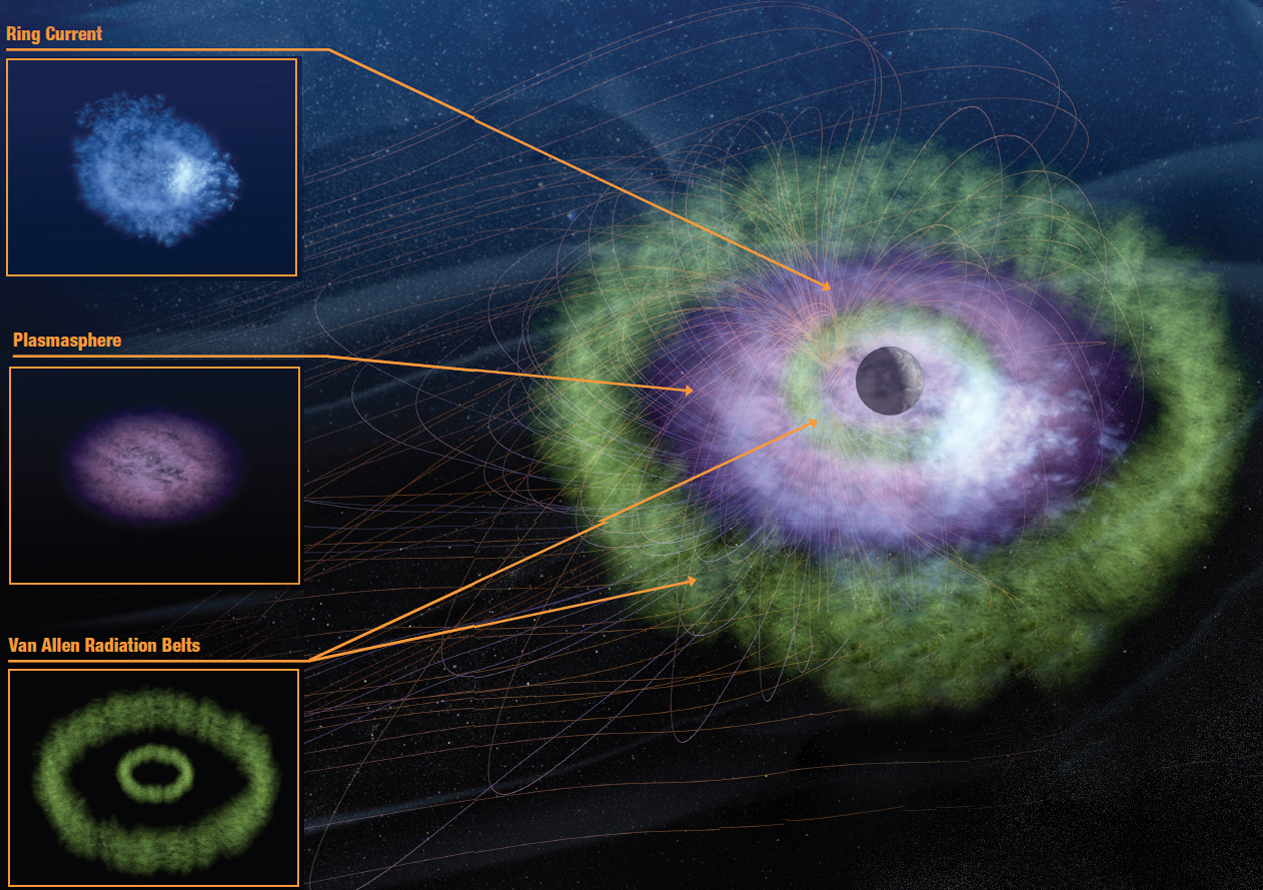
\includegraphics[scale=0.3]{{Figures/innermag-2.jpg}}
	\caption{Overview of inner magnetosphere. Adapted from \citep{InnerMagNASA}}
	\label{fig:magnetosphereoverview}
\end{figure}



\subsubsection{Processes}

The complex structure of the magnetosphere and plasmasphere leads to a number of distinct behaviors and processes such as a ring current and geomagnetic storms and substorms, all of which are driven by the solar wind.

The Ring Current, one of the major magnetospheric currents shown in Figure \ref{RingCurrentFigure}, is composed of charged particles drifting opposite directions around the Earth based on their polarity. A schematic of this from a top-down perspective is shown in Figure \ref{fig:Gold1960DriftMotion}. With enough energetic particles drifting together, a current is generated that can significantly affect the magnetic field measured on Earth's surface. These particles in the current are energized into the magnetosphere via conditions that cause the solar wind's magnetic field to reconnect with that of Earth.

\begin{figure}[htp]
	\centering
	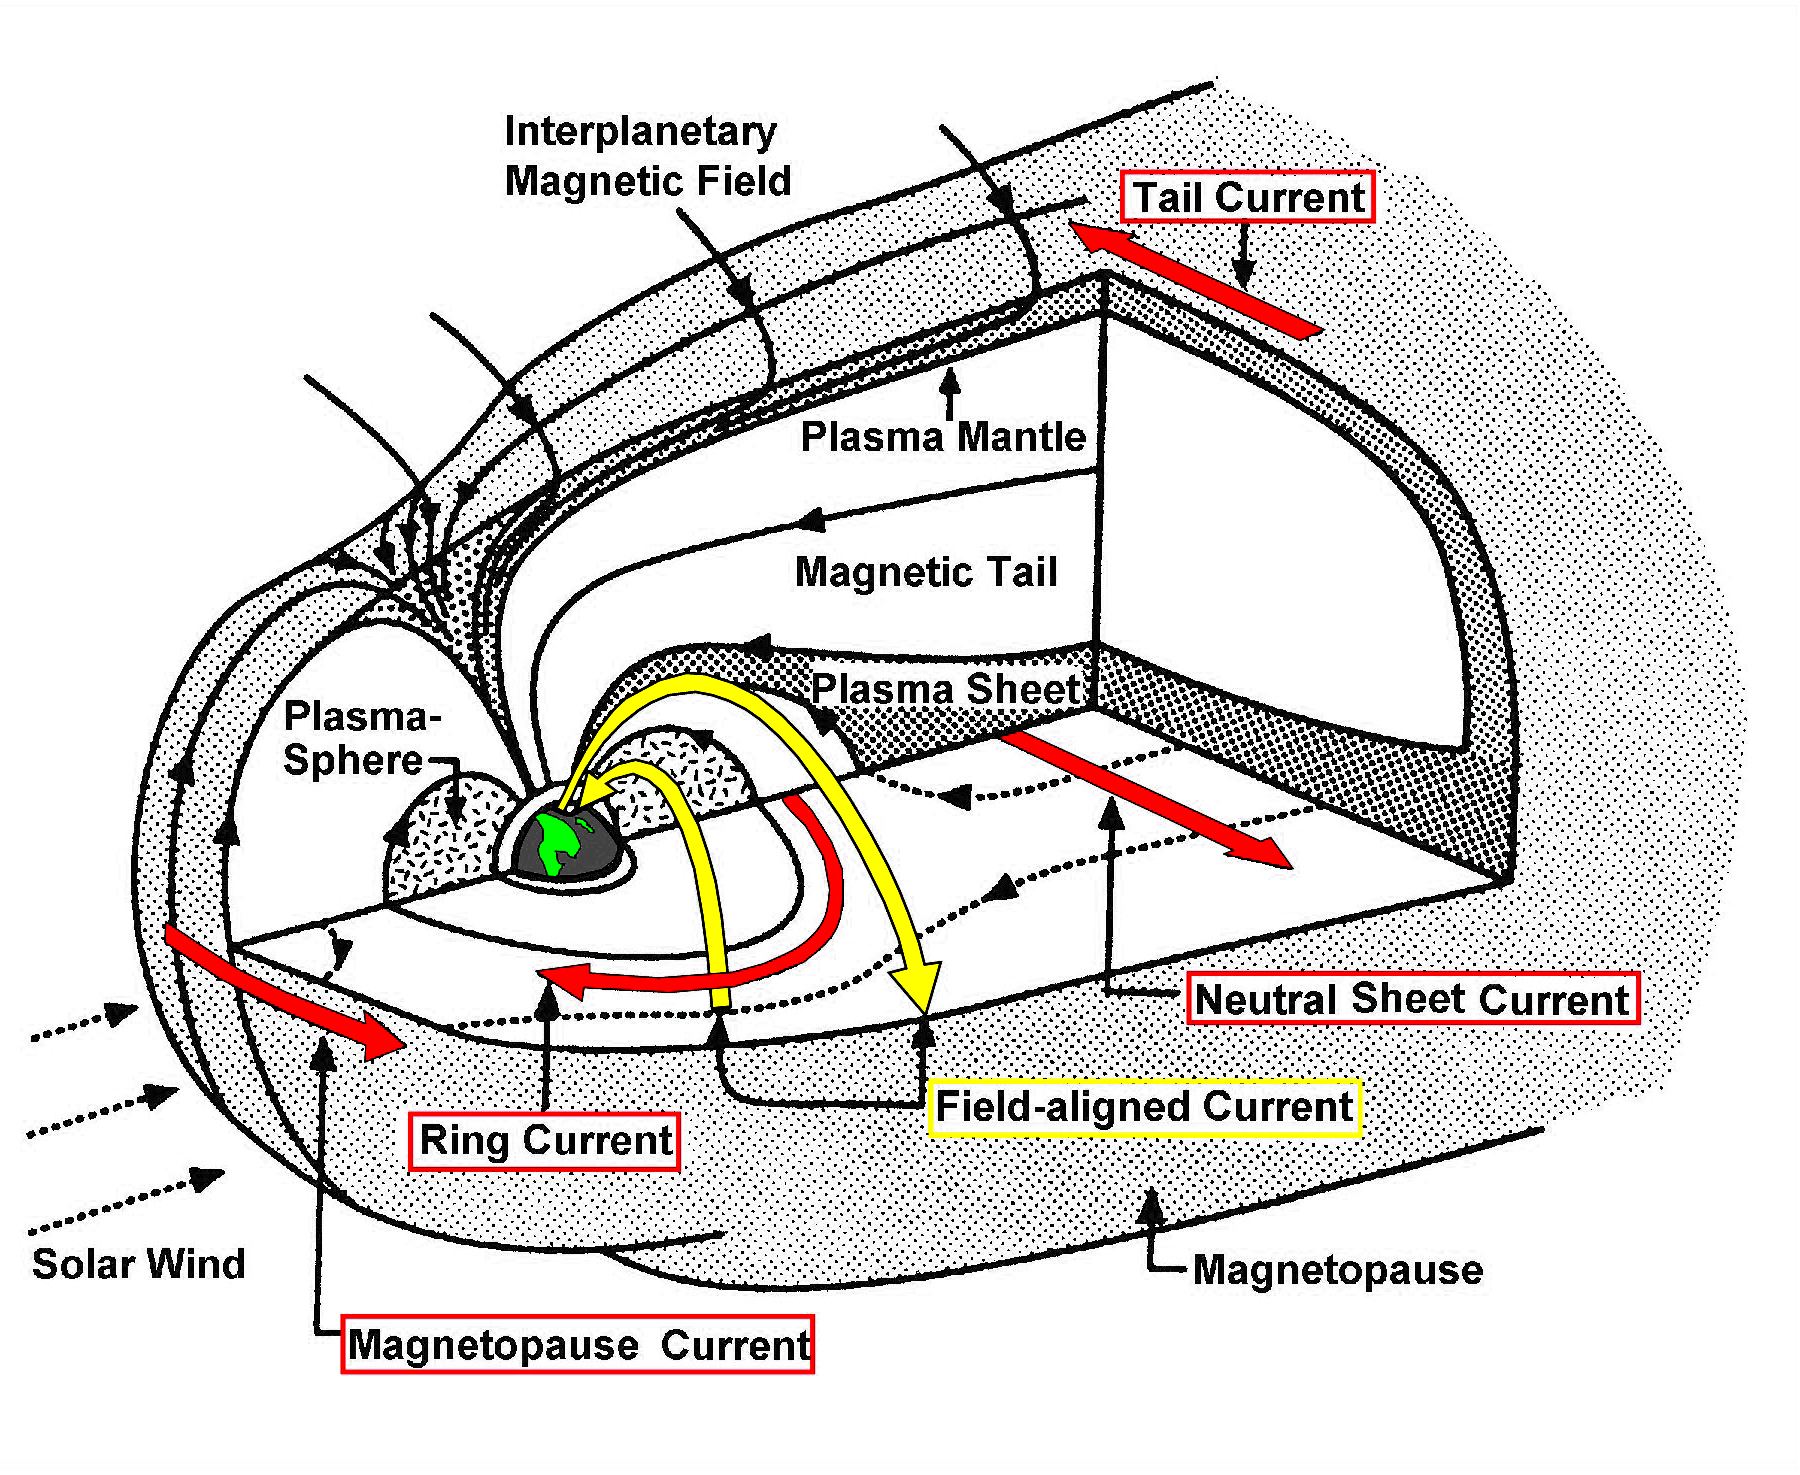
\includegraphics[scale=0.25]{{Figures/magnetosphere.jpg}}
	\caption{Currents in/around the magnetosphere. Adapted from \citep{MagnetosphereCurrentFigure}}
	\label{RingCurrentFigure}
\end{figure}


\begin{figure}[htp]
	\centering
	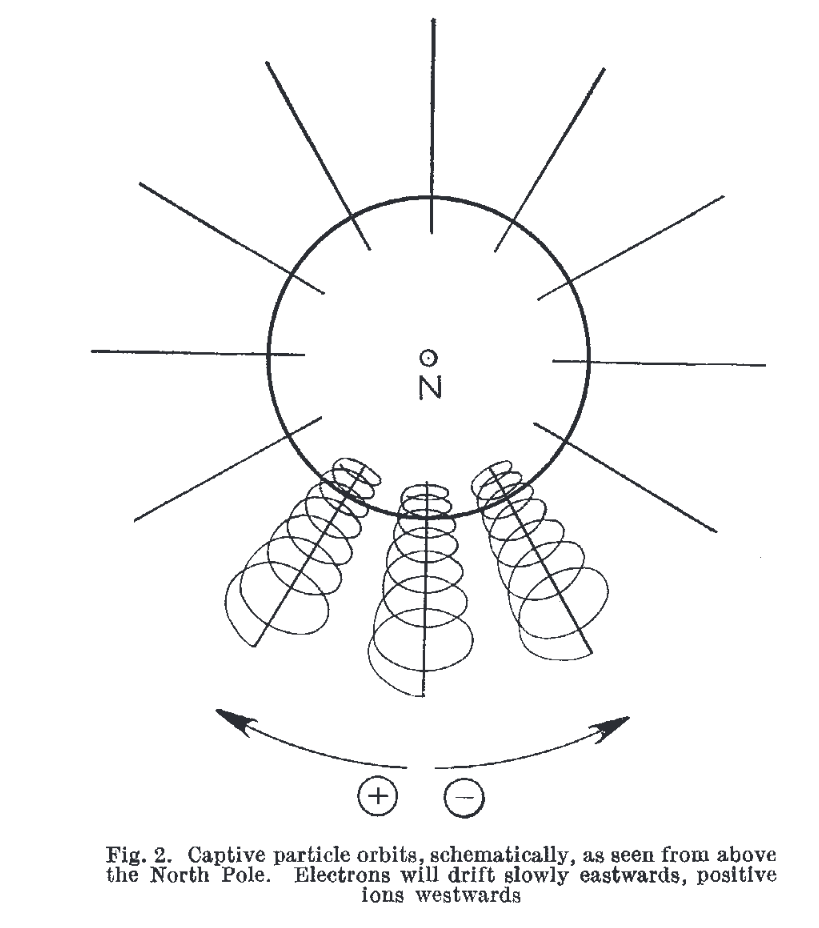
\includegraphics[scale=0.3]{{Figures/Gold1960RingCurrent.png}}
	\caption{Top-down schematic of particle drift \citep{Gold1959RingCurrent}}
	\label{fig:Gold1960DriftMotion}
\end{figure}


Geomagnetic storms occur when the solar wind interacts with the Earth's magnetosphere in such a way as to produce significant disruptions in its normal, quiet-time, behavior. A geomagnetic storm is generally defined by a significant change to the magnetic field measured by multiple ground-based magnetometer measurements from stations spread around the world, in the case of the $K_P$ index, or around the geomagnetic equator in the case of the disturbance storm-time ($D_{st}$) index. These indices are used to classify storms into categories of severity \citep{NOAAScale}. The definition of storms in the literature varies slightly between authors \citep{Yermolaev}, but most agree that sustained and abnormally perturbed near-earth and mid-to-low geomagnetic latitude magnetic field strengths over several hours or more constitutes a geomagnetic storm \citep{StormDefinition}. 

Geomagnetic substorms, in contrast with storms, are much shorter; typically only lasting for an hour or two, and potentially happening soon after one another. They tend to have a less appreciable effect on the amount of particles/energy in the ring current, and are associated with sudden changes in energy coming from the tail of the magnetosphere rather than the dayside reconnections associated with storms \citep{Gonzalez1994WhatIsAStorm}. Figure \ref{fig:alldata-GOES6-1989-1989} serves as an example of this, where a long, high-intensity storm is punctuated with a few small, short disturbances in both $B_z$ and \dst.

\begin{figure}[htp!]
	\centering
	\includegraphics[width=1\linewidth]{Figures/alldata-GOES6-10Mar1989-17Mar1989.eps}%alldata-GOES6-1989-1989}
	\caption{Data from GOES 6 around March 1989 geomagnetic storm}
	\label{fig:alldata-GOES6-1989-1989}
\end{figure}



Geomagnetic storms and substorms can have significant impacts on Earth and space systems, from inducing currents in large power grids to harming satellite circuitry and onboard data \citep{1989Storm}. Because of the potential damage of such events, any ability to forecast a storm could allow operators to prevent or mitigate problems in their systems. Because of the large correlation of CMEs with geomagnetic storms \citep{Yermolaev}, it can be estimated that our forewarning time is the difference between observing a CME (via visual or X-ray methods) and its propagation time plus magnetospheric interaction time. This time can span from one to five days, depending on the speed of the CME and how it interacts with the interplanetary medium \citep{StormSources}. 

All of these processes are coupled to some degree with the plasmasphere, by transferring plasma and energy from the interplanetary medium to near-Earth regions ($\lesssim 8 R_E$). 


\subsection{Radiation Belts}

\subsubsection{Discovery}
The radiation belts that surround Earth, known as the Van Allen Radiation Belts, are two (occasionally three \citep{LinksBetweenPlasmapauseRadiationBelt}) bands of energetic particles encircling the planet. The existence of such bands was theorized based on knowledge of magnetically trapped motion of charged particles; results from rocket soundings showed that more radiation exists in the auroral regions than at the equator.  The beginning of the space age allowed particle counters to be launched onboard the Explorer 1 and Explorer 3 satellites, which found radiation far beyond what was anticipated and concentrated into bands of high intensity \citep{MagnetoHistory}.

\subsubsection{Processes}
The outer radiation belt is filled with electrons captured from the solar wind by the magnetosphere and then injected into the radiation belts from the magnetotail, and occasionally lost when the magnetopause moves back Earthward \citep{Millan2007ReviewRadiationElectronLoss}. The inner belt tends to be filled by heavier species from the ionosphere, and is overall less variable than the outer belt \citep{LinksBetweenPlasmapauseRadiationBelt}. It gains particles from inward radial diffusion and loses them to the atmosphere via plasmaspheric hiss \citep{Lyons1973StructureRadiationBelt}. The slot region between the two is formed by the interaction of energetic particles with very low frequency (VLF) waves, leading to particle loss to the atmosphere \citep{LongTermVariationsSlotRegion}. In contrast to the ring current particles, the radiation belt particles tend to have much higher energy 

\begin{figure}[htp]
	\centering
	\includegraphics[scale=0.15]{{Figures/BounceMotion.eps}}
	\caption{Motion of magnetically trapped particles \citep{IntroductionToGeomagneticallyTrapped}}
	\label{BounceMotion}
\end{figure}

The various forms of particle movement are shown in Figure \ref{BounceMotion}. The primary component being the drift motion leading to the ring current. As particles approach the ``Mirror point", a slight angle between the guiding center motion and the magnetic field line leads to a force opposing the motion along the line, eventually mirroring the particle back in the opposite direction. Because mirroring applies to all particles within a certain range of energies and pitch angles, the collective sum of trapped particles forms the radiation belts. By modeling the particle mass, momentum, and the magnetic field strength of a given dipole magnetic field, approximations can be made regarding the amount of particles that will become trapped in the field, and the amount that will be lost to scattering \citep{Young2008MagneticFieldLineCurvature}.

The radiation belts have an impact on the plasmasphere by acting as an occasional source of low energy particles and a sink for high energy particles. The plasmasphere also acts on the radiation belts via the VLF waves, energizing electrons out of the plasmasphere and into the radiation belts, or providing particles already in the belts the energy needed to become untrapped \citep{LinksBetweenPlasmapauseRadiationBelt}. While the outer limits of the plasmasphere and the outer radiation belt often coincide and react similarly to geomagnetic activity, they can become separated during geomagnetically active times \citep{LinksBetweenPlasmapauseRadiationBelt}. An example of this variation in relative position is shown in Figure \ref{PlasmasphereRadiationBeltFig}.

\begin{figure}[htp!]
	\centering
	\includegraphics[scale=0.15]{{Figures/Cluster_plasmasphere.eps}}
	\caption{Relative position of plasmasphere (blue) and radiation belts (red) with varying geomagnetic activity levels \citep{LinksBetweenPlasmapauseRadiationBeltFig}.} 
	\label{PlasmasphereRadiationBeltFig}
\end{figure}

Another source/sink of energy for particles in the radiation belts (or general magnetospheric plasma) is via Alfvén waves \citep{Keling2009AlfvenWaves}. These waves are composed of oscillating electromagnetic fields carrying both energy and field-aligned currents (via oscillating electrons) as they propagate. By moving energy along the field lines, Alfvén waves also couple the various distinct regions of plasma around Earth. 


\subsection{Plasmasphere}

\subsubsection{Discovery}
The plasmasphere, shown in Figure \ref{fig:magnetosphereoverview}, was largely unknown until the beginning of the space age, being found both through analyses of very low frequency radio waves and in-situ spacecraft measurements. Previously, it was believed that electron density decreased continuously from the ionosphere to the interplanetary medium \citep{LemaireEarthsPlasmasphere}. These experiments showed that the Earth had a sphere of cold plasma around it that ended in an abrupt boundary, and varied in location and density gradient with geomagnetic activity \citep{Carpenter1966WhistlerStudiesPlasmapause,LemaireEarthsPlasmasphere}.

\subsubsection{Processes}
The plasmasphere is interconnected with the radiation belts and the ionosphere. While many of the specifics of this interaction are still not fully understood, some parts have been observed and explained to a reliable degree of accuracy. 

In the ionosphere, during the daytime sunlight photoionizes oxygen which produces excess electrons that are transferred up via polar wind into the plasmasphere along magnetic field lines bringing energy and heat along with it. This daily ``refilling"  flux continues until a saturation point is reached, bringing the lower bounds of the plasmasphere into equilibrium with the upper ionosphere. This flux also typically reverses on the night side, sending electrons back down into the ionosphere \citep{LemaireEarthsPlasmasphere}. Figure \ref{fig:PlasmasphereRefilling} shows one particular example of active geomagnetic conditions emptying the plasmasphere following by a quiet time refilling flux restoring density over a couple of days.

\begin{figure}[htp]
	\centering
	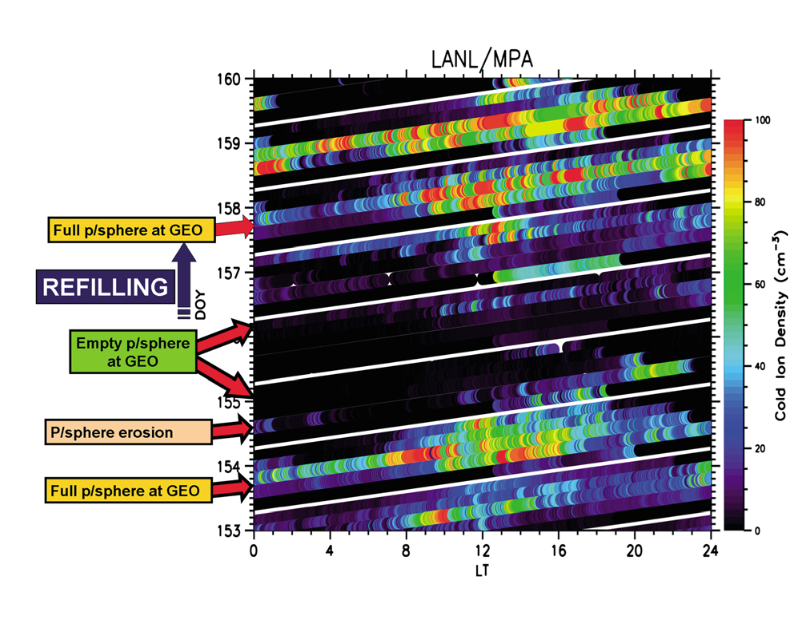
\includegraphics[scale=0.4]{{Figures/PlasmasphereRefillingT.png}}
	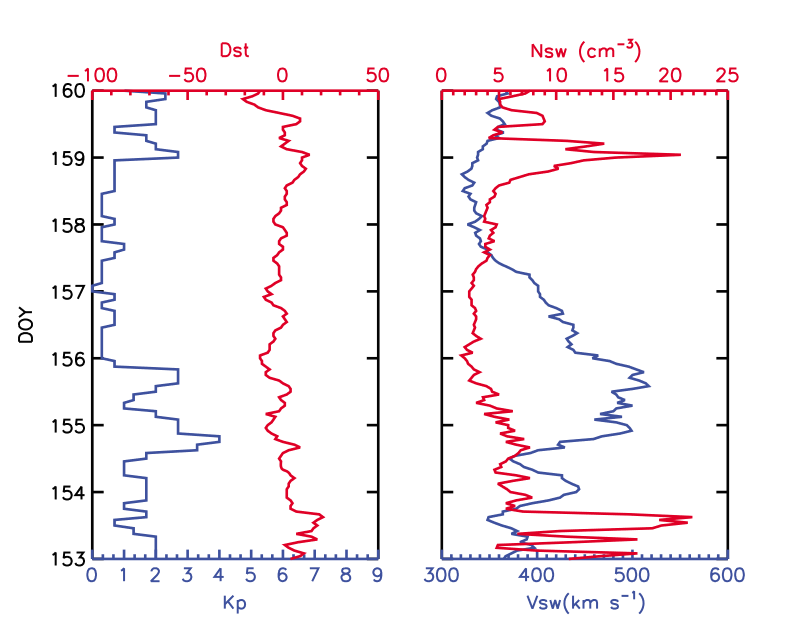
\includegraphics[scale=0.4]{{Figures/PlasmasphereRefillingB.png}}
	\caption{Plasmasphere ion density emptying and refilling as measured by GEO in 2007, along with coinciding solar wind conditions. From \citep{Denton2014ObservationsModelingRefilling}.}
	\label{fig:PlasmasphereRefilling}
\end{figure}


During periods when the location of the plasmapause is quickly brought earthwards, or the plasmapause is re-established in a new location, plasma left outside the plasmapause is known to be magnetically convected outwards and sunwards \citep{ErosionRecoveryPlasmasphere, LemaireEarthsPlasmasphere}, termed ``eroding" the plasmasphere. This is because the location of the plasmapause can vary greatly with geomagnetic conditions. Figure \ref{fig:LemaireKnee} shows how the $L$-shell distance varies with magnetic activity via the $K_p$ index.

\begin{figure}[htp]
	\centering
	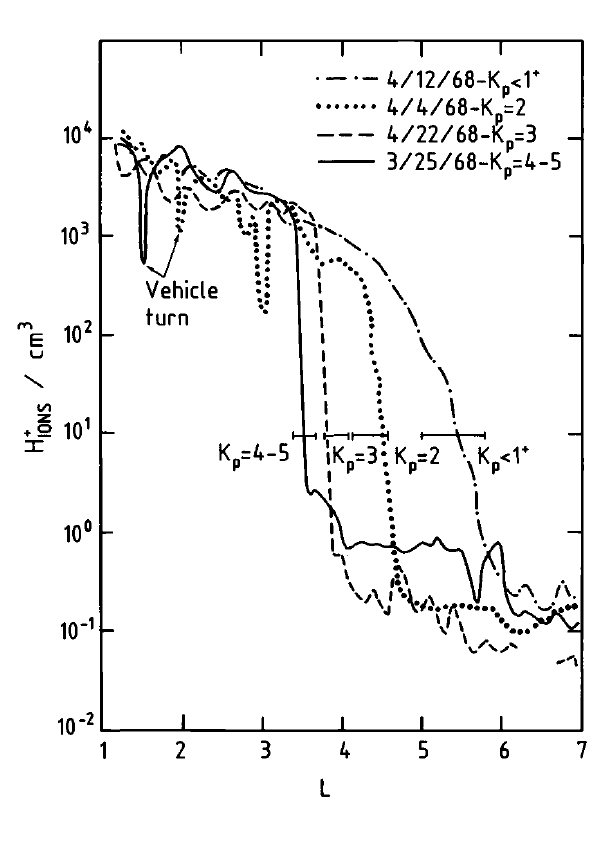
\includegraphics[scale=0.65]{{Figures/LemairePlasmapauseKnee.png}}
	\caption{Plasmapause position varying with $K_p$ as represented by several particular plasmapause crossings made on outbound passes between local times of midnight and 0400. From \citep{LemaireEarthsPlasmasphere}}
	\label{fig:LemaireKnee}
\end{figure}

Figure \ref{fig:LemaireKnee} also shows the plasmatrough; the low density region just outside the plasmapause where particle count often drops multiple orders of magnitude from the plasmasphere and continues out through the magnetosphere. The location of what is called the "plasmapause knee" varies with time and geomagnetic activity, where the dayside boundary is often less steep than the nightside boundary. It's also observed in Figure \ref{fig:LemaireNoKnee} that after multiple days of quiet geomagnetic conditions, the saturated plasmasphere smooths the knee out until the plasmapause is almost unidentifiable \citep{LemaireEarthsPlasmasphere}. 

\begin{figure}[htp]
	\centering occasional 
	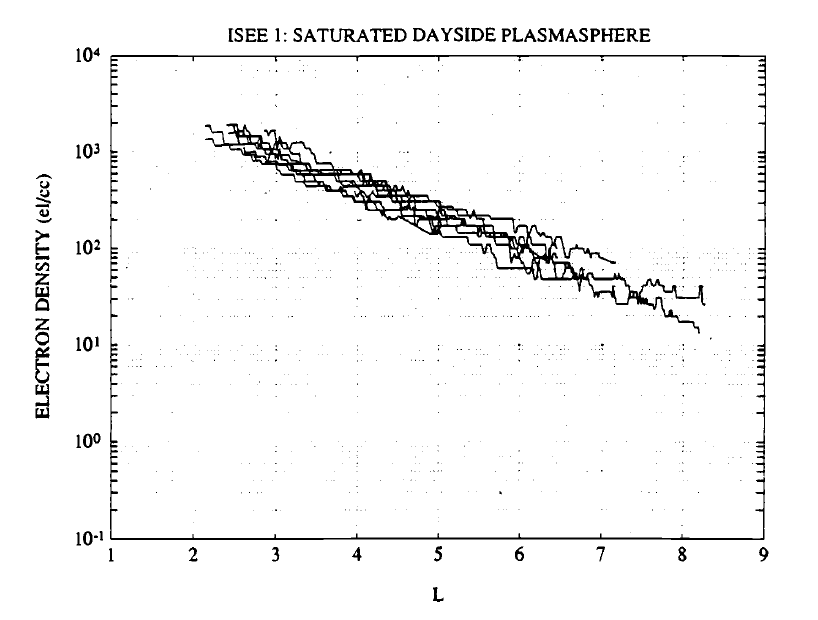
\includegraphics[scale=0.5]{{Figures/LemaireQuietPlasmapause.png}}
	\caption{Multiple ISEE 1 passes made between 09-15 MLT during saturated plasmapause conditions. From \citep{LemaireEarthsPlasmasphere}}
	\label{fig:LemaireNoKnee}
\end{figure}


At times, the plasmasphere becomes distorted at the plasmapause due to dayside reconnection, causing bulges that can become elongated and detached during co-rotation, usually on the dusk side. These extended segments of plasma are known as ``plumes" and appear as a peak in density in a normally empty plasmatrough. These plumes also often occur with, and possibly because of, enhanced magnetospheric activity \citep{EvolutionPlasmasphericIons}. This bulge, and the effects of geomagnetic activity on the bulge, is shown in Figure \ref{fig:plasmabulge}

\begin{figure}[htp]
	\centering
	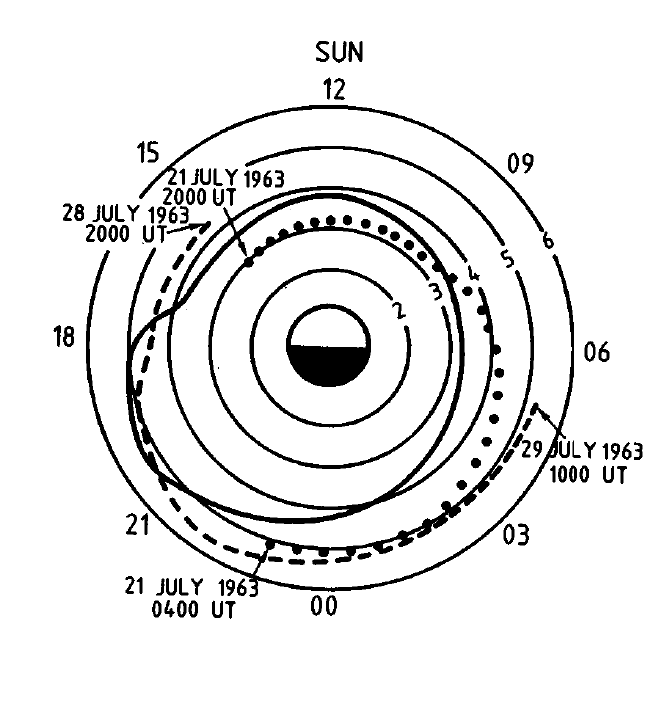
\includegraphics[scale=0.5]{{Figures/LemairePlasmapauseRadius.png}}
	\caption{Plasmasphere dusk-side bulge with geomagnetic activity. The solid line is the average position of the plasmasphere knee during periods of $K_p=2-4$, while the dots indicate a specific instance of increasing magnetic activity, and the dashes a specific instance of decreasing activity. From \citep{LemaireEarthsPlasmasphere}.}
	\label{fig:plasmabulge}
\end{figure}

What's not particularly well studied or understood is the behavior of plasma mass density in the plasmatrough. Most studies focus on behavior inside the plasmapause where density is higher and easier to measure, but since this mass diffuses inwards from the solar wind and through the plasmatrough, and satellites are often located in the plasmatrough (geostationary equatorial orbit (GEO) is at about 6-7 $R_E$), it is worthwhile understanding the behavior of the region. This work takes a dataset specifically focused on mass density in the plasmatrough and attempts to understand, classify, and forecast behavior as it relates to solar wind and geophysical conditions.


\subsection{Statistical Modeling of Magnetosphere and Plasmasphere}

Initial forecasts of geomagnetic disturbances were based on an observed time delay from sunspot sitings \citep{SunspotStorms}. The state of geomagnetic storm forecasting then advanced to a basic theory involving electromagnetic interactions in the magnetosphere \citep{Chapman}. There now exist entire services dedicated to executing statistical and magnetohydrodynamic (MHD) based models of the magnetosphere \citep{CCMC}, as well as multi-year, multi-institution efforts to survey the general statistics of modeling and forecasting of extreme events \citep{ExtremeEvents}.

The convergence of the advancement in both statistical and MHD-based simulation has led to a situation where the scientific community has the capacity for monitoring and forecasting the near-Earth effects in real time.  There have been efforts to test the forecast performance of select models over a small number of geomagnetic events \citep{ANNforecast,StormModel,StatCompStorms,Yermolaev, GEMPapers}. However no research has been done that involves the analysis of long-term forecasting performance of these models and comparison of the results with existing methods.

Three main metrics of magnetospheric activity are seen throughout the literature; the $K_p$ index: a measure of magnetosphere convection caused by currents induced by a changing plasma sheet (and indirectly from the global convection field strength) \citep{Thomsen2004WhyKpSoGood}; the $AE$ index: a measure of electrojet activity based on the maximum and minimum field strength measurements from magnetometer stations at auroral latitudes \citep{DavisSugiura1966AE}; and the previously mentioned $D_{st}$ index based on magnetic field perturbations caused primarily by a changing ring current.

\note Needs diagram showing how measurements are made

Models specific to the plasmasphere and plasmatrough include Carpenter and Anderson's ISEE/Whistler Model of Equatorial Electron Density in the Magnetosphere, which use empirical data to determine the location and density of the saturated plasmasphere and plasmatrough \citep{Carpenter1992ISEEModel}. \cite{Carpenter1992ISEEModel} analyze ISEE 1 data for drops in number density of at least a factor of 5 across half an L-shell and state that the inner edge of the plasmapause is located at $L_{ppi}=5.6-0.46K_{p_{max}}$. Here $K_{p_{max}}$ is the maximum value of $K_p$ (an index averaging 11 mid-latitude stations in the previous 24 hours), and $L$ is the set of magnetic field lines at a distance of $L$ Earth radii at the magnetic equator. This specifies the outer boundary of the plasmasphere, and from there the density is modeled inwards as $n_e=n_{e_{L_{ppi}}}\cdot 10^{-(L-L_{ppi})/\Delta pp}$, where $n_{e_{L_{ppi}}}$ relates day number, sunspot number, whistler profiles, and multiple year-long perturbations in an exponential fashion shown as $n_e(L,d,\bar{R})=10^{\Sigma x_i}$. $L_{ppi}$ and $\Delta pp$ are empirically derived plasmapause location and width, respectively. $x_1$ is a whistler reference profile, and indices $i=2-4$ represent perturbation values for annual, semiannual, and solar cycle variations respectively. The exact numbers in the density profiles vary slightly between a midnight-06 MLT model, and a 06-15 MLT model, based on the specific passes used to fit the parameters for each section. 

\cite{Gallagher2000GlobalCore} created a Global Core Plasma Model which combines empirically derived models of the ionosphere, plasmasphere, and magnetosphere. For the plasmasphere it links plasma density and magnetosphere conditions by fitting Carpenter's equation, but replacing their piecewise dependence on MLT with a sinusoidal term along with extra factors to account for the post-dusk bulge while still keeping the plasmasphere model continuous. At the most basic level, the plasmasphere component reduces to an exponential equation of the form $n_{ps}=10^{gh}-1$, where $g$ and $h$ are terms relating to the inner plasmasphere and plasmapause, combining sunspot number, day of year, and a plasmapause gradient term that accounts for the MLT dependence in the form of $\Delta_{pp}=0.036\cdot \sin(\frac{2\pi (MLT-6)}{24})+0.14$. They also link plasmasphere filling time to $K_p$, stating it starts at 3.5 MLT and fills until a time of $\Phi_{TP}=0.145K_p^2-2.63K_p+21.86$ hours \citep{Gallagher1995AzimuthalVariation}.

\cite{Moldwin2002ModelPlasmapause} build on Carpenter's model by taking CRRES data and the same plasmapause detection parameters as Carpenter, finding 969 plasmapause detections compared to the 40 used to derive the model in \cite{Carpenter1992ISEEModel}. Using the abundance of data they do statistical analyses such as showing a least squares linear fit between increasing $K_p$ and decreasing L-shell of the plasmapause of the form $L_{pp}=(5.39\pm 0.072)-(0.382\pm 0.019)\cdot K_p(max)$ with a correlation of 0.548. They also find that if they limit this to plasmapause crossings between 09 and 15 MLT, the linear correlation increases to 0.727.

\cite{OBrien2003EmpiricalPlasmapause} find that using auroral electrojet (AE) or disturbance storm time ($D_{st}$) indices work better than $K_p$ for determining plasmapause location. They use the same plasmapause crossings as \cite{Moldwin2002ModelPlasmapause} and model them against hourly changes in the ring current (via $D_{st}$) or 1-minute changes in the auroral electrojet currents ($AE$). They take the maximum (or minimum, as required) of each index over a varying range of hours, from a start of up to 72 hours before crossing up to end of at least 6 hours before crossing, and fit a basic linear model. Their three best models were a basic linear fit of $L_{pp}$ to $\text{max}_{-36,-2}K_p$, $\text{max}_{-36,0}AE$, and $\text{log}_{10}(\text{min}_{-24,0}D_{st})$. Using a bootstrap analysis for significance, all three models were indistinguishably similar in the root mean square error (RMSE) of their respective models, except for $AE$ having significantly less error in the night sector than $D_{st}$. Making the model slightly more advanced by including a MLT dependence and periodic terms allows a bulge to be approximated, and finds that the allowing local time to be accounted for significantly (at the 95\% confidence level) reduces the error of the model, but still shows no significant difference between models of the same complexity.

As for models specifically of the plasmatrough, \cite{Lotoaniu1999PlasmaMassDensity} take ground based Ultra Low Frequency (ULF) wave measurements, then map them to plasma mass densities between $L=4.5$ and $L=10$ via the Tsyganenko T89 magnetic field model and an $R^{-4}$ plasma mass density profile. These estimated values were then compared to in-situ measurements from the CRRES satellite and found that this technique can, under specific conditions where all of the field lines at the ground stations map to plasmatrough, accurately measure plasmatrough mass density. 

\cite{Takahashi2006MassDensityInferred} take a similar approach, but approximate ULF waves from the CRRES satellite directly, instead of using ground stations, and then map that to mass density values. By using the electric field spectra on the satellite and finding a fundamental frequency of the toroidal waves, they estimate mass density with a combination of theoretical model and empirical observations. The magnetic field model used is either T89 or T96, dependent on $K_p$ or \dst\  respectively. Instead of an $R^{-4}$ dependence for the mass density model, they use $\rho=\req(LR_E/R)^{0.5}$, and then combine with frequency observations via $\rho_{eq\_est}=\rho_{eq\_theory}(f_{1\_theory}/f_{1\_obs})^2$.

Most of these studies focus on plasma density in the plasmapause and plasmasphere, since that is where the densities are the highest, easiest to measure, and have the most data availability. This study focuses on the plasmatrough partly due to it's unexplored nature, and largely due to the significance of the region to objects in geostationary orbits. It also couples with both the magnetosphere and plasmasphere, suggesting that a greater understanding of the behavior of the plasmatrough may aid in understanding the coupling of both major bordering regions.


\vnote Takahashi (2010), Denton (2006, 2015), Min 2013, Tsyganenko models. Can summarize multiple papers in 1 or 2 more paragraphs. Look at O'brien and moldwin intros

\note Make connection to each paper with a section in chapter 2.


